\documentclass[]{auvsi_doc}
\setkeys{auvsi_doc.cls}{
	AUVSITitle={Summary of System Performance},
	AUVSILogoPath={figs/logo.pdf}
}

% include extra packages, if needed

\begin{document}

\begin{AUVSITitlePage}
\begin{artifacttable}
\entry{SP-001, 0.1, 04-02-19, Initial Commit, Brady Moon, Andrew Torgesen}
% additional \entry{} commands for extra rows in the revision table, if needed
\end{artifacttable}
\end{AUVSITitlePage}

% document contents (see below for LaTex commands that make your life easier)
\section{Introduction}

This artifact highlights of our testing and results for our integrated UAS. Through
a combination of simulation and hardware flight testing, we are convinced that our integrated system, together with further refinements over the next two months to maximize our point potential, will obtain a favorable market response in the AUVSI-SUAS competition. Our testing procedures and results can be distilled into four main categories: Airframe, Controls, Vision, and UGV. Summaries of these four subsystem results are detailed below.

\section{Summary of System Performance}
%Performance summary for the system, which refers to supporting artifacts as needed

%Supporting Artifacts:
%•Test results obtained using models and/or prototypes. Pay special attention to Figure 2.12 in the textbook as you consider the test results needed. Note that you will need validation testing(not just performance testing) for System Refinement approval
%•Definitions of models and/or prototypes used in testing
%•Test procedures that were used to obtain the results listed above
%•Computer files used in the testing work
%•Other detailed artifacts that support assessing the performance of the system
%•Up-to-date approved project contract, revised as necessary


\subsection{Airframe}

At the end of Fall semester, our new airframe suffered a devastating crash that left it in pieces. As a result, we confirmed the possibility of a quick two-day rebuild, and the airframe has since completed more than 20 flight tests (see Flight Log: artifact AF-004). It has successfully integrated with the imaging, autopilot, and UGV subsystems. It is light, weighing only 4.5~kg, and is spacious enough to contain all required components and more. It flies smoothly with plenty of thrust to safely take off with an endurance of approximately 50 minutes. It maintains stability despite active wind gusts of up to around 7~m/s. It flies slowly with an average flight speed around 14~m/s, resulting in crisp images and easy maneuvering. See artifact AF-001 for more detailed performance metrics.

\subsection{Controls}

\subsubsection{Stable Flight}

Thus far, over the course of numerous flight tests, we have accrued 23 minutes of autonomous flight time in hardware. Most of this autonomous hardware flight time has been for the process of tuning our autopilot gains, as detailed in artifact CT-001. The process of tuning autopilot gains has been crucial to the success of our integrated system, as it ensures stable autonomous flight. Gain tuning has resulted in excellent stability performance in the absence of wind, as well as satisfactory performance in the presence of wind.

\subsubsection{Waypoint Accuracy}

In simulation, we were able to fly waypoints within approximately 1 meter. The results were obtained through a series of 5 trials. In each trial, 5 waypoints were randomly generated and the plane was instructed to find a path that connected all 5 points. Once the path was planned, the plane flew the path in simulation. The results of the five trials are shown in Table \ref{tab:con_res}. For hardware, a similar approach was taken. Three points were located in the flight space which would be safe to fly through. Once the points were determined, the plane was commanded to plan a path through them and then fly. Due to disturbances such as wind, the plane was unable to fly the waypoints as accurately as in simulation but each waypoint was able to be flown within 5 meters. The waypoints, planned path, and flown path are shown in Figure \ref{fig:flight} in yellow, green, and white, respectively.

\begin{table}[h!]

\caption{Table of results showing the minimum distance between the UAV and each waypoint.}
\label{tab:con_res}
\begin{tabular} {|l|l|l|l|l|l|l|}
\hline
Test No. & Waypoint 1&Waypoint 2&Waypoint 3&Waypoint 4&Waypoint 5\\
\hline
1 & .750 m& .128 m& .092 m& .430 m& .688 m \\
2 & 1.058 m &.127 m & .180 m & .376 m & .328m \\
3& .602 m& .625 m&.158 m& .204 m& .122 m\\
4& .427 m & .351 m & .042 m & .018 m& 69.7m\\
5& .152 m& .085 m& .011 m & 1.11 m & .90 m\\
\hline
\end{tabular}
\end{table}

\begin{figure}
    \centering
    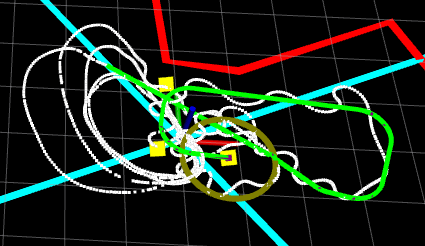
\includegraphics[width=.75\textwidth]{WaypointTest.png}
    \caption{The flight path is shown for the hardware test. The yellow points mark the desired waypoints, the green line shows the desired path, and the white line shows the actual flown path. The golden circle shows the final loiter location for the plane to fly once the planned path is flown. As a result of strong winds, the plane had difficulty staying perfectly on the planned path but was still able to follow the path and hit the waypoints.}
    \label{fig:flight}
\end{figure}

\subsection{Vision}

Through flight tests and post-flight analysis, we were able to autonomously detect 70\% of ground targets with only 1-3 false positives. Manual classification was also able to classify 100\% of targets it received during flight. The main performance bottleneck is image transfer speed from the plane to the ground. The camera is able to capture images at a high rate, but unable to stream them all back to the groundstation fast enough, causing us to loose information through flight.

For autonomous classification we were able to reliably classify 10/13 shapes and 18/26 letters. These statistics should improve as we refine our dataset and neural net models. With finetuning the day of flight, we are able to classify 7/10 colors.

\AUVSIFigure
{./figs/detection.pdf}
{\textwidth}
{Autonomous system detecting ground targets (red circles)}
{fig:autoDetection}

\subsection{UGV}

Using our new simulation and payload drop planning algorithms, we dropped our payload twice with an average
prediction accuracy of 17.7m. These drops were within our predicted performance values even though it was
a gusty day. In simulation, our payload drop planning algorithms have consistently been able to plot paths
that can drop the UGV while avoiding obstacles and competition boundaries.

\AUVSIFigure
{./figs/simulation.pdf}
{\textwidth}
{Payload Drop Plan Plot}
{fig:serverFlow}

\section{Conclusion}

Testing for obtaining key success measure values has yielded favorable results in all categories. Through hardware flight testing, we have been able to test multiple subsystems during the same flight (such as Airframe-Controls-Payload and Airframe-Vision). However, we still need to perform a mock competition for testing all key success measures in one flight during a competition setting. This will be performed in the coming days.
\end{document}
